% document formatting
\documentclass[10pt]{article}
\usepackage[utf8]{inputenc}
\usepackage[left=1in,right=1in,top=1in,bottom=1in]{geometry}
\usepackage[T1]{fontenc}
\usepackage{xcolor}

% math symbols, etc.
\usepackage{amsmath, amsfonts, amssymb, amsthm}

% lists
\usepackage{enumerate}
\usepackage{enumitem}

% images
\usepackage{graphicx} % for images
\usepackage{tikz}

% code blocks
% \usepackage{minted, listings} 

% verbatim greek
\usepackage{alphabeta}

\graphicspath{{./assets/images/Week 4}}

\title{02-614 Week 4 \\ \large{String Algorithms}}
 
\author{Aidan Jan}

\date{\today}

\begin{document}
\maketitle
\section*{Four Russian's Speedup}
There is a faster way to do edit distance than Hirschberg's algorithm that also keeps the same space complexity.
\begin{itemize}
	\item \textbf{Goal:} Edit distance faster than $O(m, n)$ with no increase in space (asymptotically).
\end{itemize}

\subsection*{Idea 1:}
Imagine we can tile our dynamic programming table with tiles of size $t$.  Instead of calculating every cell individually (and take up $mn$ time to do so), we can compute in larger chunks.
\begin{center}
% 0.8 size cells, 3.0 size tiles.
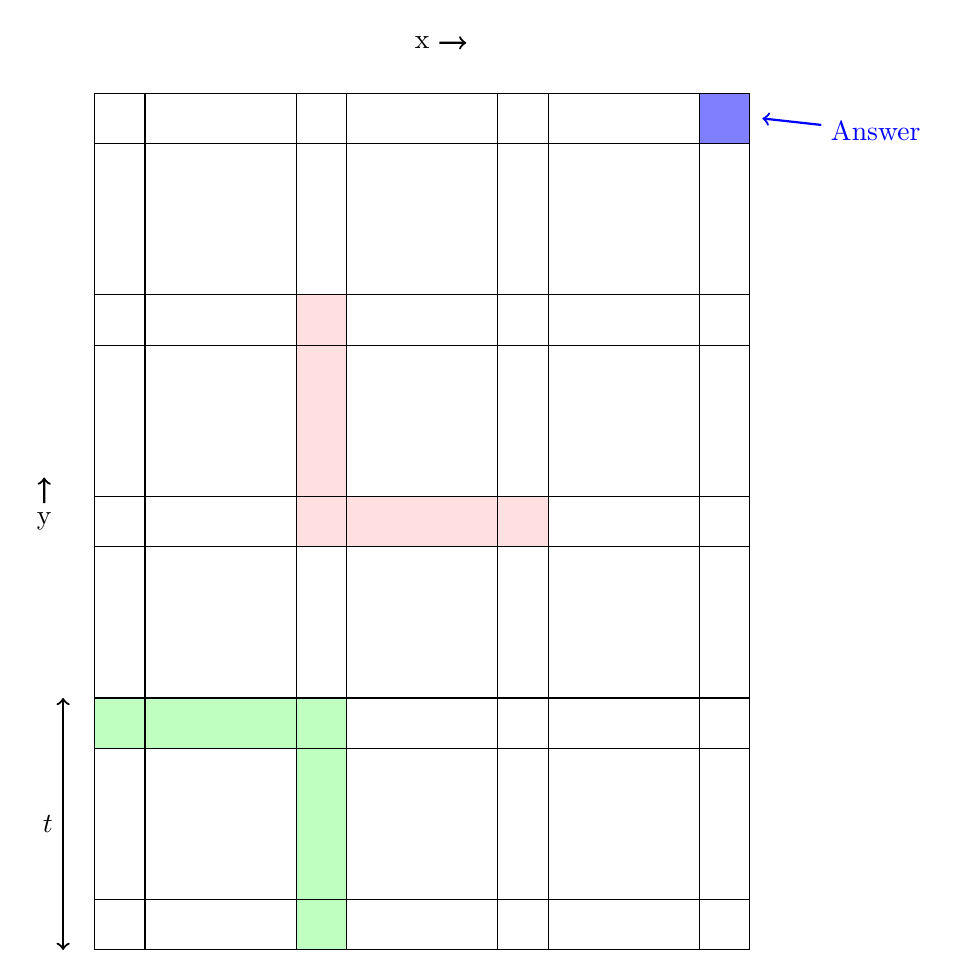
\begin{tikzpicture}[scale=0.8]
    % shading
    \fill[green!25] (3.2, 0) rectangle (4.0, 4.0);
    \fill[green!25] (0, 3.2) rectangle (3.2, 4.0);
    \fill[pink!50] (3.2, 6.4) rectangle (4.0, 10.4);
    \fill[pink!50] (4.0, 6.4) rectangle (7.2, 7.2);
    \fill[blue!50] (9.6, 12.8) rectangle (10.4, 13.6);
    % matrix
    \draw (0, 0) rectangle (10.4, 13.6);
        % vertical
        \draw (0.8, 0) -- (0.8, 13.6); \draw (3.2, 0) -- (3.2, 13.6);
        \draw (4.0, 0) -- (4.0, 13.6); \draw (6.4, 0) -- (6.4, 13.6);
        \draw (7.2, 0) -- (7.2, 13.6); \draw (9.6, 0) -- (9.6, 13.6);
        % horizontal
        \draw (0, 0.8) -- (10.4, 0.8); \draw (0, 3.2) -- (10.4, 3.2);
        \draw (0, 4.0) -- (10.4, 4.0); \draw (0, 6.4) -- (10.4, 6.4);
        \draw (0, 7.2) -- (10.4, 7.2); \draw (0, 9.6) -- (10.4, 9.6);
        \draw (0, 10.4) -- (10.4, 10.4); \draw (0, 12.8) -- (10.4, 12.8);

    % t arrow
    \draw[<->, thick] (-0.5, 0) -- node[left] {$t$} (-0.5, 4.0);

    % x / y labels
    \node at (5.2, 14.4) (x) {x};
    \draw[->, thick] (x) -- (5.9, 14.4);
    \node at (-0.8, 6.8) (y) {y};
    \draw[->, thick] (y) -- (-0.8, 7.5);

    % finish label
    \node[blue] at (12.4, 13) (fin) {Answer};
    \draw[blue, ->, thick] (fin) -- (10.6, 13.2);

\end{tikzpicture}
\begin{itemize}
	\item Each tile overlaps the other tiles by 1 row and 1 column on each side.
	\item We start from the bottom left corner (which we call cell $(0, 0)$).  Consequently, our answer is the top right.
\end{itemize}
\end{center}
First, we have to make a few assumptions:
\begin{itemize}
	\item $m = n$, or in other words, $|x| = |y|$.
	\item Our tiles exactly tile the DP matrix.
\end{itemize}

\subsection*{Idea 2:}
With this tile setup, only the edges of the tiles matter.
\begin{itemize}
	\item If we know the edges, then we don't need the centers of the tiles.
\end{itemize}
We want:
\begin{itemize}
	\item A function $f(\texttt{red shaded edges}, x', y') \rightarrow \texttt{green shaded edges}$.  In other words, take in the bottom and left edges of each tile and output the values of the top and right edges.
\end{itemize}
It turns out that we can do this using the Hirschberg or the Na\"{i}ve dynamic programming algorithm.  Therefore, a tile would take $O(t^2)$ time.  Can we compute that faster?

\subsubsection*{Computing $f$ Faster}
\textbf{Lemma:} In the edit distance (number of operations) DP matrix $D$, adjacent cells in a row, column, or diagonal differ by at most 1.
\begin{center}
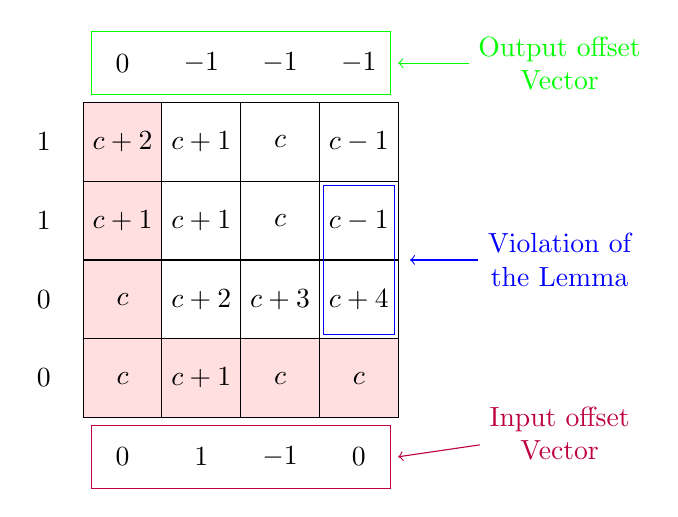
\begin{tikzpicture}
    % shading
    \fill[pink!50] (0, 0) rectangle (1, 4);
    \fill[pink!50] (1, 0) rectangle (4, 1);
    % table
    \draw (0, 0) rectangle (4, 4); 
    \draw (0, 1) -- (4, 1); \draw (0, 2) -- (4, 2); \draw (0, 3) -- (4, 3);
    \draw (1, 0) -- (1, 4); \draw (2, 0) -- (2, 4); \draw (3, 0) -- (3, 4);
    \node at (0.5, 3.5) (03) {$c+2$}; \node at (1.5, 3.5) (13) {$c+1$}; \node at (2.5, 3.5) (23) {$c$}; \node at (3.5, 3.5) (33) {$c-1$};
    \node at (0.5, 2.5) (02) {$c+1$}; \node at (1.5, 2.5) (12) {$c+1$}; \node at (2.5, 2.5) (22) {$c$}; \node at (3.5, 2.5) (32) {$c-1$};
    \node at (0.5, 1.5) (01) {$c$}; \node at (1.5, 1.5) (11) {$c+2$}; \node at (2.5, 1.5) (21) {$c+3$}; \node at (3.5, 1.5) (31) {$c+4$};
    \node at (0.5, 0.5) (00) {$c$}; \node at (1.5, 0.5) (10) {$c+1$}; \node at (2.5, 0.5) (20) {$c$}; \node at (3.5, 0.5) (30) {$c$};
    % violation
    \draw[blue] (3.05, 1.05) rectangle (3.95, 2.95);
    \node[blue, align=center] at (6.05, 2) (vl) {Violation of\\the Lemma};
    \draw[blue, ->] (vl) -- (4.15, 2);
    % left offset vector
    \node at (-0.5, 0.5) (o0) {$0$};
    \node at (-0.5, 1.5) (o1) {$0$};
    \node at (-0.5, 2.5) (o2) {$1$};
    \node at (-0.5, 3.5) (o3) {$1$};
    % bottom offset vector
    \node at (0.5, -0.5) (0o) {$0$};
    \node at (1.5, -0.5) (1o) {$1$};
    \node at (2.5, -0.5) (2o) {$-1$};
    \node at (3.5, -0.5) (3o) {$0$};
    \draw[purple] (0.1, -0.1) rectangle (3.9, -0.9);
    \node[purple, align=center] at (6.05, -0.2) (bl) {Input offset \\ Vector};
    \draw[purple, ->] (bl) -- (4.0, -0.5);
    % top offset vector
    \node at (0.5, 4.5) (0a) {$0$};
    \node at (1.5, 4.5) (1a) {$-1$};
    \node at (2.5, 4.5) (2a) {$-1$};
    \node at (3.5, 4.5) (3a) {$-1$};
    \draw[green] (0.1, 4.1) rectangle (3.9, 4.9);
    \node[green, align=center] at (6.05, 4.5) (ol) {Output offset \\ Vector};
    \draw[green, ->] (ol) -- (4.0, 4.5);

\end{tikzpicture}
\end{center}

\subsection*{Idea 3:}
Represent the \texttt{red shaded edges} and \texttt{green shaded edges} as offset vectors.
\begin{itemize}
	\item In the example above, we define the bottom offset vector at $(0, 1, -1, 0)$, since those are the differences between each of the values in the cells along the bottom rows
	\item Since every tile represents matching a substring between $x$ and $y$ and the bottom row and left columns represent the previous alignment, the best alignment (the output) always remains the same if the input offset vectors and the characters in the string are the same.
	\item This means we can precompute every $f$ value and do lookups to fill in the edges of tiles on the DP table.
\end{itemize}
\subsection*{Idea 4:}
Precompute every possible $f$ value.
\begin{enumerate}[label=(\arabic*)]
	\item There are $3^{2(t - 1)} \cdot |\Sigma|^{2t}$ possible inputs to $f$.
	\begin{itemize}
	    \item $3^{2(t - 1)}$ comes from the fact that offset vectors must contain either $\{-1, 0, 1\}$ in each position, and there are a total of $2(t - 1)$ positions along the left and bottom sides of a tile.
	    \item The $|\Sigma|^{2t}$ comes from the number of possible substrings that could be in $x$ and $y$, for $2t$ characters total, and each character has $|\Sigma|$ choices.
    \end{itemize}
	\item Computing all possible values takes $O((3|\Sigma|)^{2t} \cdot t^2)$.  (The $t^2$ is from the DP algorithm to fill in the cells of a tile once.)
\end{enumerate}
However, the trick here is that $t$ is an arbitrary tile size value, which we are able to set.  We pick $t = \frac{1}{2}\left(\log_{3|\Sigma|}n\right)$.
\begin{itemize}
	\item Now, if we plug in for $t$, our time complexity becomes $O(n (\log n)^2)$.
\end{itemize}
This pre-computation now takes less time than the rest of the problem because we only do it once.

\subsubsection*{Storing $f_s$}
We make a tree that encodes the input and stores the output at the leaves.
\begin{itemize}
	\item Start at the root
	\item The first $2(t - 1)$ layers are all the possible offset vector combinations
	\item The next $2t$ layers are possible substrings.
	\item The output offset vectors (i.e., the top and right sides of each tile) are the data stored at the leaf nodes.
\end{itemize}
With this, searching up an $f$ value is linear time, since our tree is $O(t)$ layers deep.
\begin{itemize}
	\item In this case, the tree acts similarly to a hash map except without the $O(1)$ lookup.  It maps an input key (input offset vectors and substrings) to an output value (output offset vectors).
	\item We don't use a hash map because the number of keys we have is exponential - a hash map would run into bucketing problems and become linear time (relative to the number of total possible inputs, i.e., exponential) lookup.
	\item The search time for a tree of $O(t)$ height would be $O(t)$, which is faster than all the other parts of the algorithm anyways.
\end{itemize}

\subsubsection*{Storing the Tree}
When we store using the tree, traversing the tree takes $O(t) = O(\log n)$ time.
\begin{itemize}
    \item However, instead if we create a table (a direct map from the input to the output), we can do constant time lookup.
    \item It turns out that $O(\log(n))$ bitstrings can be manipulated in $O(1)$ time.  
    \item Every possible bitstring $O(2^{\log(n)}) = O(n)$ is stored in the table, with an $n$-sized table.
\end{itemize}


\subsection*{Total Running Time}
\begin{itemize}
	\item We have $n^2 / t^2$ tiles.
	\item It takes $O(t)$ to solve each tile by using lookups in the tree.
	\item The preprocessing takes $O(n \log^2 n)$ time.
\end{itemize}
In total, we have $O(\frac{n^2}{t^2} \cdot t + n \log^2 n)$, which simplifies to $O(\frac{n^2}{t} + n\log^2 n)$.  Since the size of $t$ we determined is equal to $\log n$, we can substitute that in, and drop the second term.  (The $\frac{n^2}{\log(n)}$ term dominates.)
\[\boxed{O\left(\frac{n^2}{\log n}\right)}\]

\subsection*{Traceback Path}
\begin{itemize}
    \item We traceback similarly to the na\"ive DP algorithm
    \item When calculating each of the tiles, we use the na\"ive algorithm, which means we also have the traceback arrows.
    \item Therefore, we can map each output position of a tile to an input position.  This adds a constant amount of storage and can be stored in the same table.
    \item In the worst case, the traceback passes through $\frac{2n}{t} = O\left(\frac{2n}{\log n}\right)$ tiles, which involves going straight left then straight down.
    \item To find the exact traceback pack, we then run the na\"ive DP algorithm only on the tiles that we pass through.  The result is $O(\frac{2n}{t} \cdot t^2) = O(n \log n)$ time.  (This term is dropped because the rest of the algorithm is slower.)
\end{itemize}

\section*{Multiple Sequence Alignment}
Suppose we multiple sequences we want to align with each other.  We can place these sequences into a matrix where each row is one string.  This matrix is referred to as the \textbf{alignment matrix}.
\begin{itemize}
	\item The goal of this alignment matrix is to add gaps to each string (so they all become the same length), and maximum \texttt{score}
	\item \texttt{colcost()} is a function that takes in a \textit{column} of the alignment matrix and returns a number, the \texttt{score}, where in general, better aligned columns score higher than misaligned columns.  Depending on the purposes of doing the alignment, this scoring function may differ.
\end{itemize}

\subsection*{\texttt{OPT} Matrix Calculation}
\[\texttt{OPT}[i_1, i_2, \dots, i_p] = \min \begin{cases}
\texttt{colcost}(\_, c, c, \dots, c) + \texttt{OPT}[i_1, i_2 - 1, i_3 - 1, \dots, i_p - 1] \\
\texttt{colcost}(c, \_, c, \dots, c) + \texttt{OPT}[i_1 - 1, i_2, i_3 - 1, \dots, i_p - 1] \\
\vdots \\
\texttt{colcost}(\_, \dots, \_, c) + \texttt{OPT}[i_1, i_2, \dots, i_{p - 1}, i_p - 1]
\end{cases}\]

\begin{itemize}
	\item Essentially, the optimal for a given cell is equal to the minumum on the $p$-dimensional DP table of (score of column from inserting gaps at certain positions) plus the optimal based on the neighboring positions.
	\item If we inserted a gap at the given row in the alignment matrix, we use the \texttt{OPT} cell at the current row.  If we don't insert a gap (represented by $c$ in the \texttt{colcost} function above), we use the previous row.
	\item In total, the \texttt{OPT} recursive function would contain $O(2^p)$ rows, since we have that many possible ways to add gaps on a given column.
	\item It is similar to running single sequence alignment on every string, except we now need to consider every string at the same time.
    \item Note that this means this problem is NP-Hard in most formulations, because computing the DP matrix would take $\Omega(n^p 2^p)$ time.  This number is hard to reduce.  However, we may use approximation algorithms for a polynomial time solution, even though they cannot offer us the optimal score.
\end{itemize}

\subsection*{Heuristic: Progressive Alignment}
Instead of aligning all the strings at the same time, we can instead align each string separately.
\begin{itemize}
	\item Call the first string $s_c$.
	\item We first run edit distance between $s_c$ and $s_2$, which may introduce gaps in either string.  Importantly, this maps every character in $s_2$ to a character in $s_c$.
	\item Then, we run edit distance between $s_c$ and $s_3$, which may introduce gaps in either string.  This provides a mapping between $s_3$ and $s_c$.  However, transitively, we also get a mapping from $s_3$ to $s_2$.
	\item We keep repeating this process with each string.  By the end, we have a mapping between every string, which can be used to rebuild an alignment matrix.
	\item Note that $s_c$ does not have to be $s_1$.  In fact, we want to choose the best $s_c$, since a different ``center'' string would change the mappings.  Most approximation algorithms using this heuristic focus on finding the best $s_c$.
\end{itemize}

\section*{Star MSA Approximation Algorithm}
\subsubsection*{Definitions}
\begin{itemize}
	\item Let $d_M(s_i, s_j)$ represent the cost of the alignment between sequences $s_i$ and $s_j$ \textbf{implied by $M$}.
	\item Let $a(s_i, s_j)$ represent the cost of the optimal pairwise alignment between $s_i$ and $s_j$.  (This is just edit distance between the two strings.)
\end{itemize}
These are not the same.  Consider the example $S = \{AT, A, T, AT, AT\}$.
\begin{verbatim}
Opt (a) between A and T:   | d_M between A and T:
                           |   
   A                       |    A-
   |  (mismatch)           |    ||   (double gap insertion)
   T                       |    -T
\end{verbatim}
We do the double gap insertion with $d_M$ because the rest of the strings would pull the $A$ to the left and $T$ to the right.

\subsubsection*{Assumptions}
\begin{enumerate}
	\item $d_M(s_i, s_j)$ has the form
	\[d_M(s_i, s_j) = \sum_{(u_i, v_j) \in M} \text{cost}(u_i, v_j)\]
    \item $\text{cost}(u, v) < \text{cost}(u, w) + \text{cost}(w, v)$
    \item $\texttt{SP-score}(M) := \sum_{i < j} d_M(s_i, s_j)$.  In other words, the score of the entire matrix is the sum of all $d_M$ pairings.
\end{enumerate}

\subsubsection*{STAR algorithm}
\begin{enumerate}
	\item Build all $O(p^2)$ \texttt{OPT} pairwise alignments
	\item Choose $s_c$ to be the input string that minimizes
	\[\sum_{i \neq c} a(s_c, s_i)\]
    \item Do progressive $d$ with $s_c$ as anchor
\end{enumerate}
We call this the STAR algorithm because by picking an $s_c$ and aligning all the other strings to it, it looks like a star if each string is a node on the graph.
\begin{itemize}
	\item An edge on the STAR graph between nodes representing $s_i$ and $s_c$ would be $a(s_c, s_i)$.
\end{itemize}
Note that with this formulation, \texttt{SP-score} is like the sum of every possible stars (divided by 2 since all edges are double-counted).
\begin{itemize}
    \item \texttt{SP-score} is a clique containing all the nodes (or all strings)
	\item ``like'' the sum because \texttt{SP-score} edges represent $d_M(s_i, s_j)$, not $a(s_i, s_j)$.
\end{itemize}

\subsubsection*{Theorem:}
\begin{itemize}
	\item \texttt{STAR} represents the \texttt{SP-score} of $M$ returned by the STAR algorithm
	\item \texttt{OPT} represents the \texttt{SP-score} of $M^*$ optimal.
	\item $\frac{\texttt{STAR}}{\texttt{OPT}} \leq 2$
\end{itemize}
\textbf{Proof:}
We want to prove that
\begin{itemize}
	\item $\texttt{STAR} \leq 2B$
	\item $\texttt{OPT} \geq B$
\end{itemize}
We know by definition that
\[2 \cdot \texttt{STAR} = \sum_{i, j} d_{\texttt{STAR}}(S_i, S_j)\]
The sum part is the pairwise alignment implied by \texttt{STAR}.  From here we can simplify:
\begin{align*}
    &\leq \sum_{i \neq j} \left[d_{\texttt{STAR}}(S_i, S_c) + d_{\texttt{STAR}}(S_c, S_j)\right] & \text{(by triangle inequality)} \\
    &= \sum_{i \neq j} a(S_i, S_c) + a(S_c, S_j) & \text{(alg. did progressive alignment anchored at $S_c$)} \\
    &= 2\sum_{i \neq j} a(S_i, S_c) \\
    &= 2\sum_i \sum_j a(S_i, S_c) \\
    &= 2 \sum_i a(S_i, S_c) \sum_j 1 \\
    &\leq 2p \sum a(S_i, S_c) & \text{($p$ is the number of sequences)}
\end{align*}
The above inequality is greater than $2 \cdot \texttt{STAR}$, so the $2$ at the beginning cancel out.
\[\texttt{STAR}\leq p\sum a(S_i, S_c)\] 
This is saying that the STAR algorithm can't give you worse than $p$ copies of the alignment.\\\\
Now, define 
\[B = \frac{1}{2} p \sum_i (S_i, S_c)\]
therefore,
\[\Rightarrow \texttt{STAR} \leq 2B\]
Now, we consider the optimal alignments.
\begin{align*}
    2 \cdot \texttt{OPT} &= \sum_{i, j} d_{\texttt{OPT}} (S_i, S_j) \\
    &\geq \sum_{i, j} a(S_i, S_j)
    \intertext{The above is true because the optimal pairwise alignment, \texttt{OPT}, cannot be better than the optimal overall alignment, $a$.}
    &= \sum_i \sum_j a(S_i, S_j) \\
    &\geq \sum_i \sum_j a(S_i, S_c) & \text{The star centered at $c$ is the optimal star} \\
    &= p \sum_i a(S_i, S_c)
\end{align*}
Now, recall that this above expression is equal to $2 \cdot \texttt{OPT}$, so we can again, divide both sides by 2.
\[\frac{1}{2} p \sum_i a(S_i, S_c)\]
This is equal to $B$, as defined before.  Therefore, both $\texttt{STAR} \leq 2B$ and $\texttt{OPT} \geq B$, and $\frac{\texttt{STAR}}{\texttt{OPT}} \leq 2$.



\end{document}